\begin{figure}[h]
    \centering

    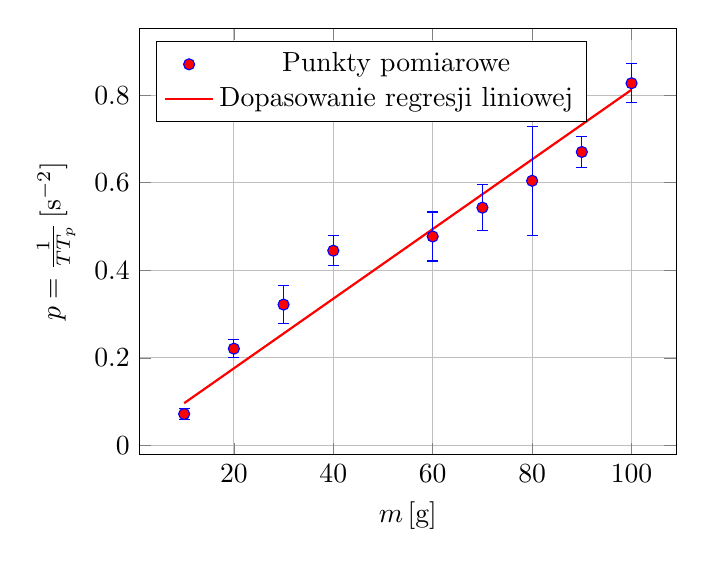
\begin{tikzpicture}
        \begin{axis}[
            width=8.4cm, height=7cm,
            xlabel={$m \, [\mathrm{g}]$},
            ylabel={$p = \frac{1}{T T_p} \, [\mathrm{s}^{-2}]$},
            legend pos=north west,
            grid=major
        ]

        \addlegendimage{only marks, mark=*, blue, mark options={fill=red}, error bars/.cd, y dir=both, y explicit}
        \addlegendentry{Punkty pomiarowe}
        
        \addlegendimage{no markers, red, thick}
        \addlegendentry{Dopasowanie regresji liniowej}
        
        \def\slope{0.00795279}
        \def\intercept{0.01695}
        
        \addplot [red, thick, domain=10:100, forget plot] {\slope*x + \intercept};
        \addlegendentry{Dopasowanie regresji liniowej}
    
        \addplot+[
            only marks,
            mark=*,
            blue,
            mark options={fill=red},
            forget plot,
            error bars/.cd,
            y dir=both,
            y explicit,
        ] table [x=x, y=y, y error=err] {
            x   y       err
            10	0.07179	0.0121
            20	0.22102	0.02113
            30	0.32161	0.04316
            40	0.44478	0.03382
            60	0.47714	0.05592
            70	0.54298	0.05218
            80	0.60435	0.12436
            90	0.67012	0.03491
            100	0.82715	0.04442
        };
        \addlegendentry{Punkty pomiarowe}
    
        \end{axis}
    \end{tikzpicture}

    \caption{Masy $m_i$ wraz z odpowiadającymi im średnimi wartościami wyrażenia $p = \frac{1}{T T_p}$, policzonymi niepewnościami standardowymi $u(p)$ oraz dopasowaniem krzywej $y = ax + b$ uzyskanej dzięki regresji liniowej.}
    \label{img:regresja_wykres}
\end{figure}
    